\documentclass[a4paper,12pt]{article} % тип документа

% report, book

% Рисунки
\usepackage{graphicx}
\usepackage{wrapfig}
\usepackage{mathtext}
\usepackage[left=2cm,right=2cm,
    top=2cm,bottom=2cm,bindingoffset=0cm]{geometry}

\usepackage{hyperref}
\usepackage[]{float}
\usepackage[rgb]{xcolor}
\hypersetup{				% Гиперссылки
    colorlinks=true,       	% false: ссылки в рамках
	urlcolor=blue          % на URL
}

%  Русский язык

\usepackage[T2A]{fontenc}			% кодировка
\usepackage[utf8]{inputenc}			% кодировка исходного текста
\usepackage[english,russian]{babel}	% локализация и переносы


% Математика
\usepackage{amsmath,amsfonts,amssymb,amsthm,mathtools} 


\usepackage{wasysym}

\author{Сидорчук Максим Б01-204}
\title{2.2.3 Измерение теплопроводности воздуха при атмосферном давлении}
\date{}
\begin{document}
\maketitle
\section{Цель} Измерить коэффициент теплопроводности воздуха при атмосферном
давлении в зависимости от температуры.
\section{Оборудование} Цилиндрическая колба с натянутой по оси нитью; термостат;
вольтметр и амперметр (цифровые мультиметры); источник
постоянного напряжения; реостат (или магазин сопротивлений).
\section{Теоретические сведения}
Теплопроводность - это процесс передачи тепловой энергии от нагретых
частей системы к холодным за счёт хаотического движения частиц среды (молекул, атомов и т.п.). Закон Фурье:
\begin{equation}
	\overrightarrow{q}=-\kappa\cdot \nabla T
\end{equation}
$\overrightarrow{q}$ - плотность потока энергии, $\kappa \backsim \lambda\bar{\upsilon}\cdot nc_v$ - коэффицент теплопроводности.
Для цилиндрической геометрии (рис. \ref{цилиндр})
\begin{figure}[H]
	\begin{center}
		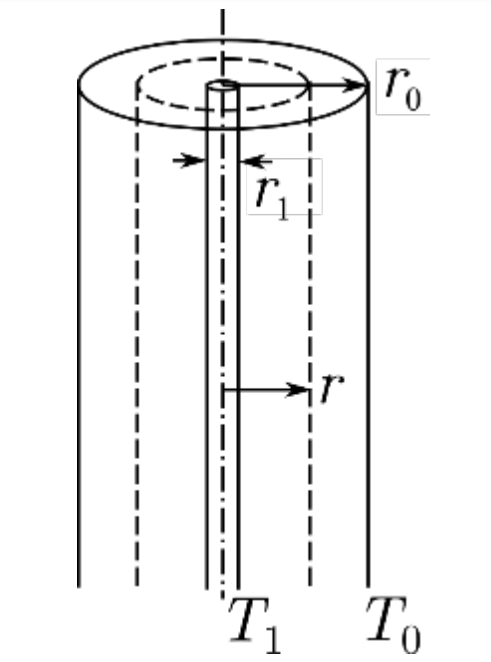
\includegraphics[width=0.3\textwidth]{Цилиндр}
	\end{center}
	\caption{Геометрия измерений} \label{цилиндр}
\end{figure}
Для стационарного режима и малого перепада температуры между нитью и стенками цилиндра:
\begin{equation}
	Q = -2\pi r L\cdot \kappa \frac{dT}{dr}=\frac{2\pi L}{ln\frac{r_0}{r_1}}\kappa\cdot \Delta T
\end{equation}

\section{Экспериментальная установка и методика измерений}
Схема установки представлена на рис. \ref{схема}. Полость трубки заполнена воздухом при атмосферном давлении, металлическая нить - источник тепла и датчик температуры. Электрическая схема установки на рис. \ref{электричество}
\begin{figure}[H]
	\begin{center}
		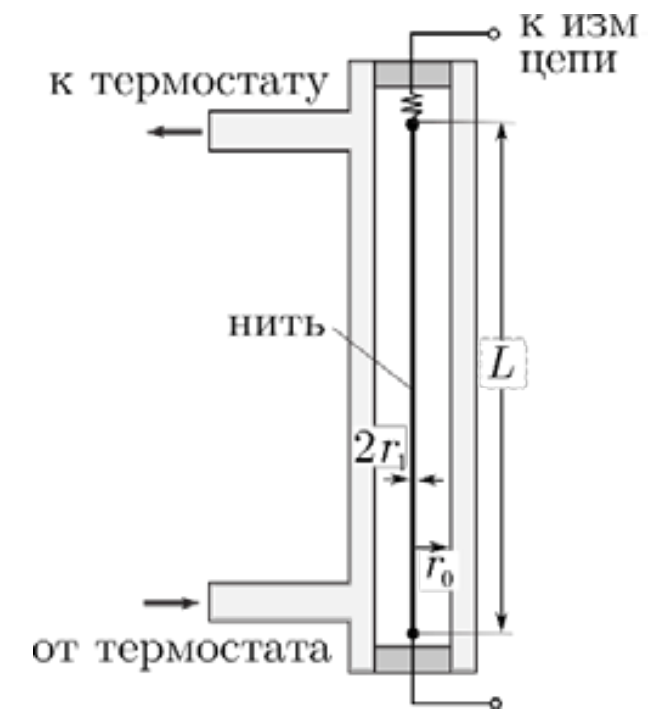
\includegraphics[width=0.3\textwidth]{Схема}
	\end{center}
	\caption{Схема установки} \label{схема}
\end{figure}

\begin{figure}[H]
	\begin{center}
		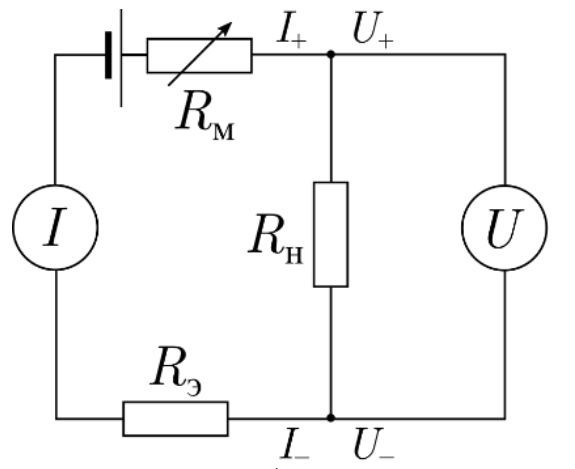
\includegraphics[width=0.3\textwidth]{Электричество}
	\end{center}
	\caption{Электрическая схема установки} \label{электричество}
\end{figure}
Ток цепи регулируется с помощью магазина сопротивлений, включенного последовательно с источником напряжения.

Измерение нагрузочных кривых позволяет получить температурную зависимость сопротивления нити (при $Q \to 0$, $T\approx T_0$)

Для исследуемых температур:
\begin{equation}
	R(t)=R_{273}\cdot(1+\alpha t)
\end{equation}
$\alpha=\frac{1}{R_{273}}\frac{dR}{dT}$  - температурный коэффициент сопротивления материала. По наклонам нагрузочных кривых можно получить значение коэффициента теплопроводности.

\section{Измерения и обработка данных}
Результаты измерений представлены в таблице \ref{результаты}.
\begin{table}[H]
	\caption{Результаты измерений}
	\label{результаты}
	\begin{tabular}{|c|c|c|c|c|c|c|c|c|c|c|c|}
		\hline
		\multicolumn{2}{|c|}{$T = 297$ K} & \multicolumn{2}{|c|}{$T = 303$ K} & \multicolumn{2}{|c|}{$T = 308$ K} & \multicolumn{2}{|c|}{$T = 313$ K} & \multicolumn{2}{|c|}{$T = 323$ K} \\ \hline
		$U$, мВ & $I$, мА & $U$, мВ & $I$, мА & $U$, мВ & $I$, мА & $U$, мВ & $I$, мА & $U$, мВ & $I$, мА \\ \hline
		218.0  & 10.8399  & 215.2  & 10.4727  & 219.0  & 10.4750 & 222.7  & 10.4773 & 217.5  & 10.0010 \\ \hline
		429.0  & 21.2783  & 430.7  & 20.9276  & 438.3  & 20.9357 & 445.8  & 20.9302 & 435.7  & 20.0030 \\ \hline
		643.0  & 31.8114  & 647.3  & 31.3537  & 658.4  & 31.3384 & 669.8  & 31.3549 & 656.1  & 30.0140 \\ \hline
		857.0  & 42.2430  & 866.8  & 41.7930  & 880.9  & 41.7642 & 895.3  & 41.7402 & 876.8  & 40.0070 \\ \hline
		1081.0 & 52.9298  & 1087.2 & 52.1480  & 1104.9 & 52.1063 & 1124.2 & 52.1435 & 1101.9 & 50.0413 \\ \hline
		1527.0 & 73.6798  & 1311.0 & 62.4825  & 1334.0 & 62.5326 & 1355.0 & 62.4739 & 1329.0 & 60.0319 \\ \hline
		1732.0 & 82.8991  & 1771.0 & 83.0506  & 1564.0 & 72.7582 & 1591.0 & 72.8143 & 1559.0 & 69.9339 \\ \hline
		1969.0 & 93.3041  & 2008.0 & 93.2471  & 1799.0 & 82.9729 & 1830.0 & 83.0501 & 1799.0 & 80.0707 \\ \hline
		2207.0 & 103.4000 & 2250.0 & 103.3453 & 2044.0 & 93.3470 & 2074.0 & 93.2044 & 2040.0 & 89.9312 \\ \hline
		 &  &  &  & 2290.0 & 103.4776 & 2330.0 & 103.5982 & 2287.0 & 99.9344 \\ \hline
	\end{tabular}
\end{table}
Для всех температур построим график зависимости сопротивления нити от мощности. (рис. \ref{нагрузка}). Из графиков получаются следующие значения (табл. \ref{обработка})
\begin{figure}[H]
	\begin{center}
		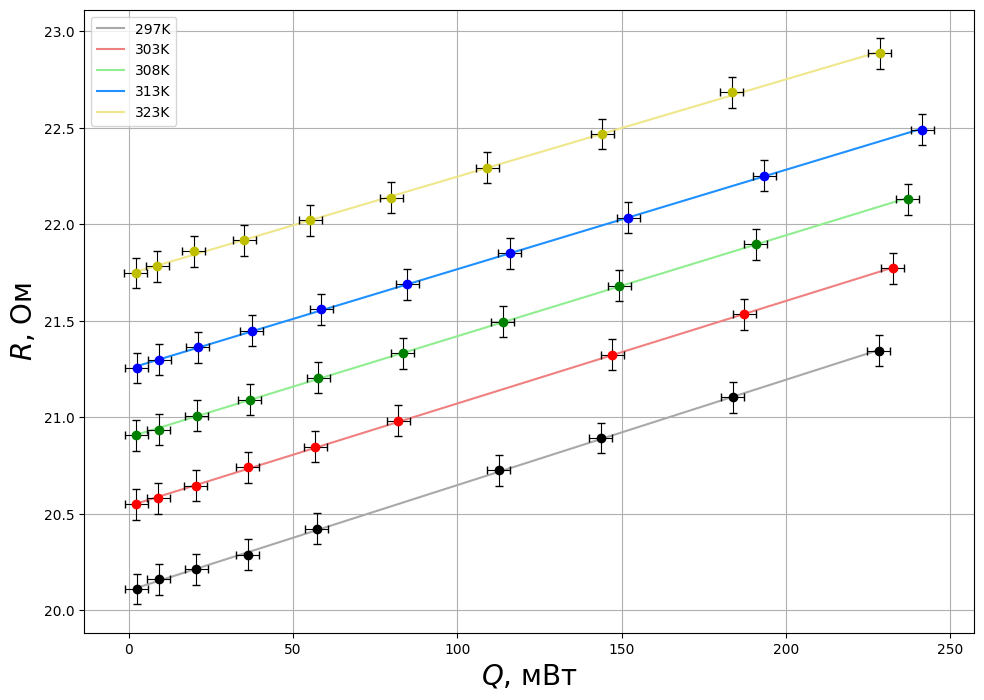
\includegraphics[width=\textwidth]{Нагрузка}\end{center}
	\caption{Нагрузочные кривые для различных температур} \label{нагрузка}
\end{figure}

\begin{table}[H]
	\caption{Результаты обработки данных}
	\label{обработка}
	\begin{tabular}{|c|c|c|c|c|c|}
		\hline
		$T$, K          & 297    & 303    & 308    & 313    & 317\\ \hline
		$R/Q$, мОм/мВт  & 5.46 & 5.31 & 5.23 & 5.15 & 5.04 \\ \hline
		$\sigma_{R/Q}$, мОм/мВт & 0.23 & 0.23 & 0.22  & 0.22 & 0.21 \\ \hline
	\end{tabular}
\end{table}

Построим график зависимости сопротивления нити от её температуры (рис. \ref{R(T)})
\begin{figure}[H]
	\begin{center}
		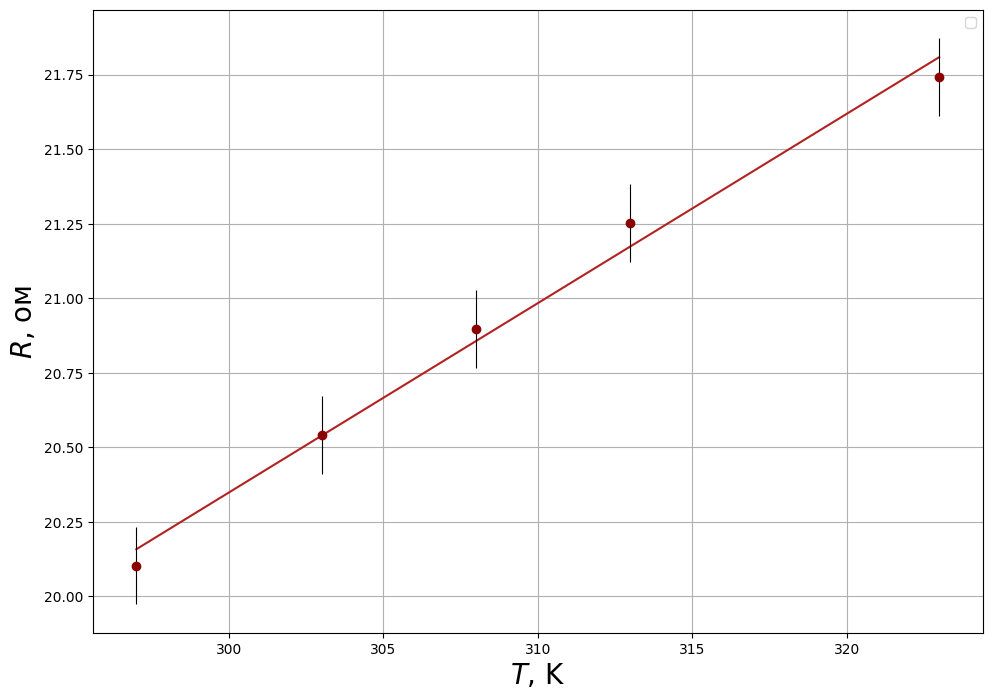
\includegraphics[width=\textwidth]{R(T)}\end{center}
	\caption{Зависимость сопротивления от температуры} \label{R(T)}
\end{figure}
Погрешность на графике заметна, но не чересчур велика, что указывает на приемлемое качество измерений.

Из графика и линейной зависимости сопротивления от температуры найдем температурный коэффициент сопротивления:
\begin{equation}
	\alpha=\frac{1}{R_{273}}\frac{dR}{dT}=(3.3 \pm 0.7)\cdot 10^{-3}  1/К
\end{equation}

Используя полученное значение и нагрузочные кривые, получим коэффицент теплопроводности для разных температур (табл. \ref{кси})

\begin{table}[H]
	\caption{Коэффициент теплопроводности для разных температур}
	\label{кси}
	\begin{tabular}{|c|c|c|c|c|c|}
		\hline
		$T$, K                     & 297   & 303   & 308   & 313 & 323   \\ \hline
		$\kappa$, мВт/(м$\cdot$K)        & 21.86 & 22.9 & 24.09 & 25.09 & 25.90 \\ \hline
		$\sigma_\kappa$, мВт/(м$\cdot$K) & 0.40 & 0.42 & 0.44 & 0.43 & 0.44 \\ \hline
	\end{tabular}
\end{table}

Погрешности полученных значений заметны, но не критичны. На приведенном ниже графике четко видна линейная зависимость.

\begin{figure}[H]
	\begin{center}
		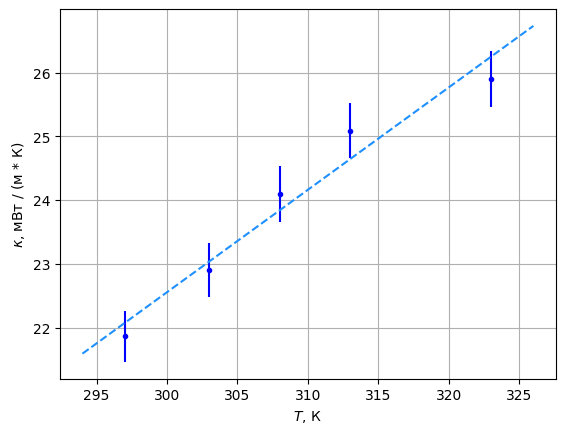
\includegraphics[width=\textwidth]{kappa.png}\end{center}
\end{figure}

\section{Выводы}

\hspace{5mm}
1. Получен линейных характер нагрузочных кривых, рассчитаны значения сопротивления при $Q=0$ и коэффицент наклона прямой.

2. Получен температурный коэффициент сопротивления: $\alpha=(3.3 \pm 0.7)\cdot 10^{-3}  1/К$.

3. Получена явная линейная зависимость $\kappa$ от температуры с коэффицентом $\frac{dQ}{d(\Delta T)} = (0.16 \pm 0.01)$.
\end{document}